
% JuliaCon proceedings template
\documentclass{juliacon}
\setcounter{page}{1}
\usepackage{flushend} % don't know if this will work...
\begin{document}

% **************GENERATED FILE, DO NOT EDIT**************

\title{A Data Persistence Architecture for the SimJulia Framework}

\author[1]{Van Der Paelt Piet}
\author[1]{Lauwens Ben}
\author[2]{Signer Beat}
\affil[1]{Royal Military Academy, Renaissancelaan 30, Brussels, Belgium}
\affil[2]{WISE Lab, Vrije Universiteit Brussel, Pleinlaan 2, Brussels, Belgium}

\keywords{\mbox{Discrete-Event Simulation}, \mbox{Frameworks}, \mbox{Tools}, \mbox{Data Storage}, \mbox{Persistence}, \mbox{Julia}, \mbox{ConcurrentSim}, \mbox{ResumableFunctions}, \mbox{PostgresORM}, \mbox{Object-Relational Mapping}, \mbox{Metaprogramming}, \mbox{Macro Expansion}}

\hypersetup{
pdftitle = {A Data Persistence Architecture for the SimJulia Framework},
pdfsubject = {JuliaCon 2022 Proceedings},
pdfauthor = {Van Der Paelt Piet, Lauwens Ben, Signer Beat},
pdfkeywords = {\mbox{Discrete-Event Simulation}, \mbox{Frameworks}, \mbox{Tools}, \mbox{Data Storage}, \mbox{Persistence}, \mbox{Julia}, \mbox{ConcurrentSim}, \mbox{ResumableFunctions}, \mbox{PostgresORM}, \mbox{Object-Relational Mapping}, \mbox{Metaprogramming}, \mbox{Macro Expansion}},
}


\maketitle

\begin{abstract}
Simulation software users run simulated models to decide on problems that are generally too difficult to solve analytically. The probabilistic elements in such simulations necessitate multiple runs, which in turn generate data. This data is of key importance for the user since it is used to decide upon the questions the simulations were run for in the first place. To enable transcendence in time and space for this data, the requirement for the end user to be familiar with persistence technology is of utmost importance, but not always present. In this work, we present a solution to this contradiction. We present a novel transparent data persistence architecture as an extension of the ConcurrentSim package. We integrated \texttt{PostgresORM.jl} into the \texttt{ResumableFunctions.jl} and \texttt{ConcurrentSim.jl} packages by using Julia's metaprogramming support. As such, we were able to remove the dependency on a user's knowledge on architectures for persistence. Furthermore, we implemented two distinct approaches to externalise the data. The first one is oriented towards a REST API, which can be consumed by existing frameworks and application templates. The second one integrates our dynamic object-relational mapping (ORM) in the existing \texttt{VueJS.jl} package.  Our contribution aims to improve the usability of the \mbox{ConcurrentSim} ecosystem, whilst demonstrating the power of macro expansion to move towards a dynamic ORM configuration.
\end{abstract}

\section{Introduction and Motivation}\label{Intro}

The rationale behind simulation is to collect data on systems or processes that are more likely to be described by a model which can be evaluated numerically, rather than being subject to exact mathematical methods which produce an analytic solution~\cite{law2007simulation}. Therefore, the goal is to generate data by means of simulation which in turn allows for conclusions to be drawn on the system from which the model originated.\vskip 6pt

Abar~et~al. \cite{abar2017agent} consider an extensive list of Agent-Based Modelling and Simulation (ABMS) tools, both open-source and proprietary. A categorisation, amongst others, on the model development effort is made. Furthermore, Abar states \textit{"An ideal simulation system should require minimal learning effort as well as provide flexible support to creating models and running robustly on any type of computing machine."} We share that thought. Moreover, since ConcurrentSim  is a process-oriented framework, in which a simulated entity can be seen as an independently coded agent, ConcurrentSim  merits its place amongst other ABMS tools as considered by Abar. \vskip 6pt

We feel Abar's statement can be extended to the monitoring and persistence aspect. To the best of our knowledge, none of the open-source frameworks provide an easy-to-implement data storage mechanism. It is our observation that monitoring creates an additional burden for an end user due to the dependency on knowledge of technology for persistence and how to interact with it from within the simulation model, regardless of the chosen programming language or implementation. Our goal is to lower that burden by removing this dependency. \vskip 6pt

We focus on the ConcurrentSim  \cite{lauwens2017simjulia,lauwens2017simjuliaSite} Discrete Event Simulation (DES) framework implemented in the Julia Programming Language \cite{bezanson2017julia}. This framework is highly inspired by SimPy \cite{SimPy} and DISCO \cite{helsgaun1980disco}, which is a SIMULA \cite{DahlNygaard1966simula} class for combined continuous and discrete simulation. The framework has been adopted in diverse research projects situated in several domains, including the Medical (\textit{SIMEDIS: a Discrete-Event Simulation Model for Testing Responses to Mass Casualty Incidents} \cite{de2018simedis}), Human Resources (\textit{Manpower planning using simulation and heuristic optimization} \cite{abdessameud2019manpower}), Ballistics (\textit{Simulating a Stochastic Differential Equation Model by Exact Sampling} \cite{hermosilla2017ballistics}) and Network Dynamics Modeling (\textit{QuantumSavory.jl: A multi-formalism simulator for noisy quantum communication and computation hardware} \cite{QuantumSavory})\vskip 6pt

Currently, ConcurrentSim  lacks the functionality to transparently store state variables which characterise the evolution of a running DES model as well. To mitigate this shortcoming, we extended both the \texttt{ConcurrentSim.jl}  \cite{lauwens2017simjulia,lauwens2017simjuliaSite} and the \texttt{ResumableFunctions.jl} \cite{lauwens2017resumablefunctions} packages by implementing a transparent probing and data persistence architecture, employing Julia's metaprogramming support. The high-level architecture of our implementation is depicted in Figure \ref{fig:highlevelarch}.
\begin{figure}[th]
	\centering
	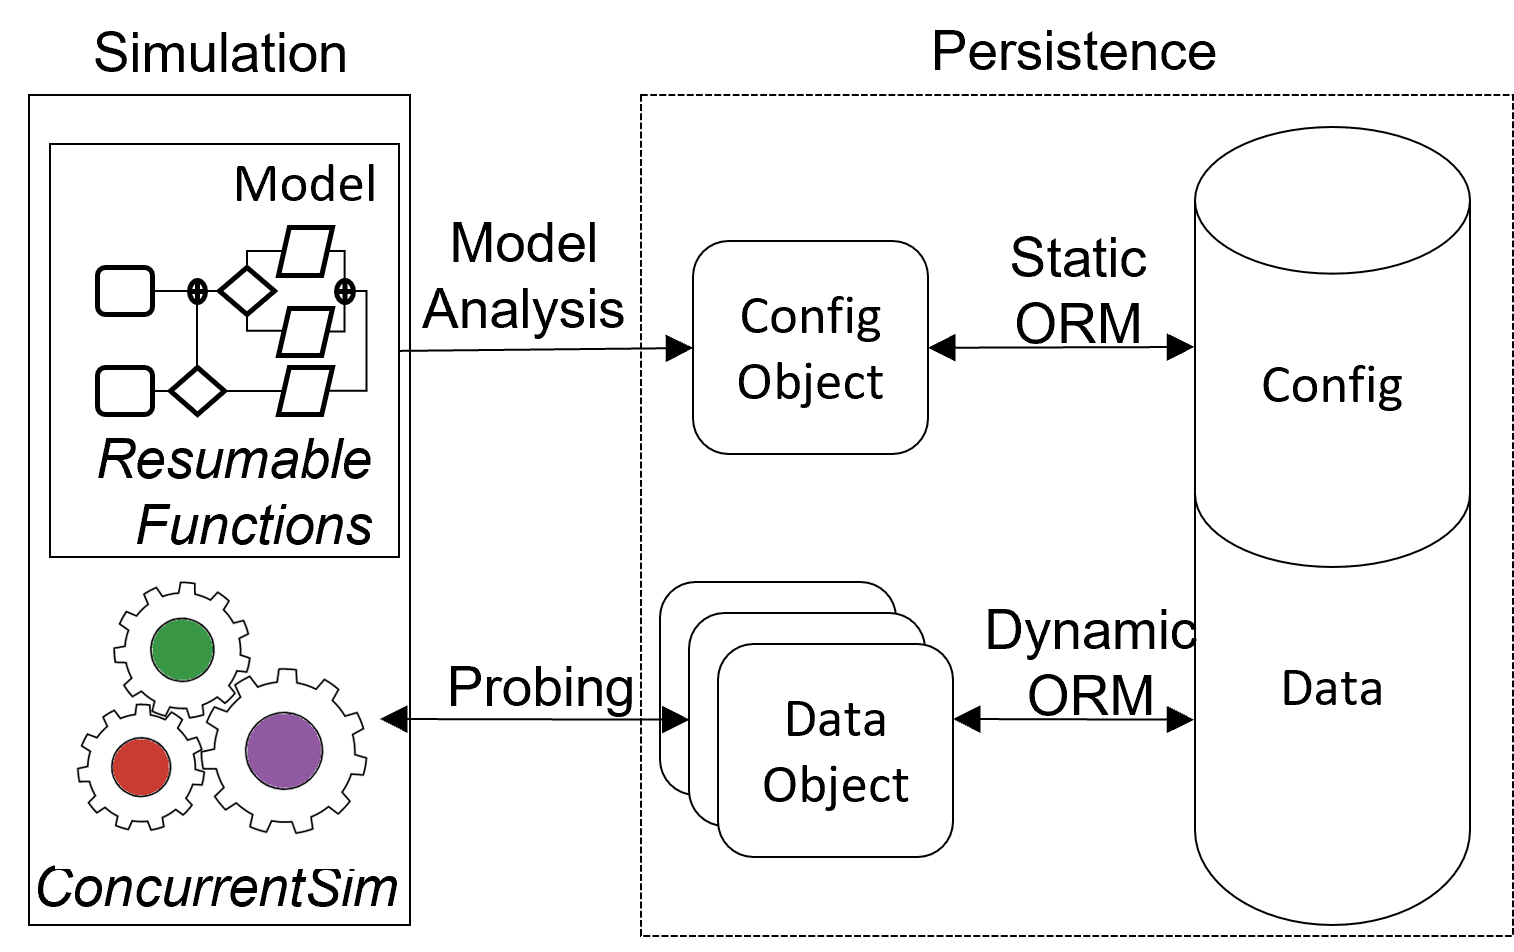
\includegraphics[width=0.9\linewidth]{images/HighLevelArch}
	\caption{Persistence: High-level Architecture}
	\label{fig:highlevelarch}
\end{figure}

At high level, we distinguish a static phase, during which model analysis takes place trough a modification of \texttt{ResumableFunctions.jl}, from a dynamic phase, during which a simulated system is probed to retrieve generated data by employing an added callback function in the \texttt{ConcurrentSim.jl}  package. To store the data, both phases use the Object Relational Mapping (ORM) concept \cite{russell2008bridging} implemented in the \texttt{PostgresORM.jl} package \cite{tecnivelPostgresORM}, supported by the PostgreSQL Relational Database Management Systems (RDBMS) \cite{psqldocs}. \vskip 6pt

We start by providing an overview of related work, in which, amongst others, we present the three main packages having a central role in our work. This is followed by the presentation of our architecture for probing and persistence in \texttt{ConcurrentSim.jl} simulations. The technical evaluation describes use cases and recorded outcome. The subsequent discussion section explains the rationale behind important decisions and choices we made. Finally, we conclude on the acquired improvements through our architecture. \vskip 6pt

\section{Related Work}\label{MainPackages}

Booth~et~al. categorise persistent data as data that outlives the application, both in time and space \cite{booch2008object}. Once data is generated in a object-oriented model, it must remain available in a data container for later use. Often, in contemporary applications this data container is an RDBMS. Ireland~et~al. describe what is known as the \textit{"Impedance Mismatch Problem"}, in particular for the object-relational case, and summarise ORM as a technique to address this problem \cite{ireland2009classification}. According to Russel~et~al., an ORM is made up out of \textit{"domain classes"} and a \textit{"persistence API"} \cite{russell2008bridging}.\vskip 6pt

A historic counter example of an RDBMS used as a data container can be found in the db4o Java library, which is an object-oriented database. As described by Hauser~et~al. \cite{hauser2011review}, it illustrates another approach to solve the Object-Relational Impedance Mismatch problem. Object classes can immediately be stored to the database provider without any further intervention. Albeit capable of running in a two-tier client-server mode, the system, for which support has ended since 2014, was not to be seen as an alternative to RDMBS.\vskip 6pt

The Jakarta Persistence API (formerly Java Persistence API, JPA) provides a well-maintained alternative. Saeed~et~al. \cite{saeed2022persistence} discuss the tree main aspects that make up the API. Data Modelling concerns the annotations necessary to transform Plain Old Java Objects into Entities. Data persistence treats how instances of these entities can be stored in the underlying RDBMS. Lastly, \emph{data querying} is about retrieval of the persisted objects using a dedicated query language. Closely related is the Hibernate ORM \cite{hibernate}. Despite it is a native implementation, it is also an implementation of the JPA specification.\vskip 6pt

Diverting away from the pure object-oriented programming languages, and more towards Julia, we turn our attention to \texttt{DataFrames.jl} \cite{Dataframes}, which is the preferred method of working with tabular data in Julia, and \texttt{JuliaDB.jl} \cite{JuliaDB}, which is a persisted tabular data package through CSV files. The latter shares a lot of \texttt{DataFrames.jl}'s properties, however none of these two solutions solve the Object-Relational Impedance Mismatch problem and we consider them inappropriate for our purpose.\vskip 6pt

A promising alternative seems to be \texttt{SearchLight.jl}, which is the ORM backend for \texttt{Genie.jl}, a package for Model-View-Controller web applications in Julia. Both are part of the \mbox{Genie~Framework~\cite{genie}}. SearchLight disposes~of~implementation libraries which attach it to MySQL, Postgres and SQLite databases. As such it seems versatile. However, in practice it is very tightly coupled to Genie. The segregation of the domain object definitions and persistence API is implemented, but each separate type needs its own module for both the object definition and persistence API.\vskip 6pt

The impedance mismatch problem between object-oriented data models implemented in Julia applications and PostgreSQL RDBMS is addressed by Laugier~et~al. in their \texttt{PostgresORM.jl} package \cite{tecnivelPostgresORM}. As put forward by Russell \cite{russell2008bridging}, PostgresORM relies on a Julia module providing the Object classes and a Julia module providing the persistence API. Lauwens~et~al. created the \mbox{\texttt{ResumableFunctions.jl} \cite{lauwens2017resumablefunctions}} and \mbox{\texttt{ConcurrentSim.jl} \cite{lauwens2017simjulia,lauwens2017simjuliaSite}} Julia packages on which the simulation applications which are the target of our architecture rely on.\vskip 6pt

We strongly believe there is a gap that needs to be filled when it comes to the persistence of data originating from simulation applications. ConcurrentSim and ResumableFunctions are in an evolved state, as proven by its adoption in other simulation research projects \cite{de2018simedis,abdessameud2019manpower,hermosilla2017ballistics}. PostgresORM could provide a statically configured persistence interface to an RDBMS. However in such a scenario, Abar's concerns about learning effort and model creation \cite{abar2017agent}, which we extended to the monitoring and persistence aspect, remain valid. Therefore, we decided to implement a transparent architecture where the concern is mitigated through an automated probing and persistence mechanism. In the remainder of this section we present these three Julia packages which are most important to grasp more in detail.\vskip 6pt

\subsection{ResumableFunctions.jl}

ResumableFunctions.jl implements the macro's \texttt{@resumable} and \texttt{@yield} which transform plain Julia functions in functions which can be interrupted during evaluation with the possibility to be resumed afterwards.\vskip 6pt

The argument of the \texttt{@resumable} macro is a function definition, which, in the context of this work, represents a process we want to simulate. Several internal functions rewrite the argument-function's body. The resumable character is essentially realised through the substitution of the \texttt{@yield} macro by a return statement, followed by a label to which the iterator can jump to upon resuming execution. This new body constitutes the definition of a finite-state machine. Using \mbox{\texttt{MacroTools.jl} \cite{macrotools}}, it is integrated in a function which, when called, results in the Finite Sate Machine Interface (FSMI). That FSMI is subsequently assigned to a field in a callable mutable struct which also contains the variables included in the FSMI, and a field which holds the current state of that FSMI. Lastly, a function definition is generated which bears the same signature as the original argument-function. \vskip 6pt

A first call to that new function leads to the initialisation of the callable mutable struct, including the creation of the FSMI instance. The return of this function call is the instantiated callable struct. Subsequent calls to this returned callable struct step through the finite-state machine, causing state variables to get updated. Finally the end-state is reached. \vskip 6pt

\subsection{ConcurrentSim.jl}

Previously known as \texttt{SimJulia.jl}, \texttt{ConcurrentSim.jl}  is the event-driven simulation framework which we extended with automated persistence features. A simulated system consists of processes which are defined as (nested) resumable functions, and a simulation environment. The latter holds the datastructures containing necessary to run the simulation. The simulation environment is a mandatory argument to each of the resumable functions. \vskip 6pt

The top-level process is initialised through an instantiation of its corresponding callable mutable struct as an argument to the \texttt{@process} macro in the global scope. Other processes can be nested in functions as well by means of the \texttt{@process} macro in a local function scope. Having defined the simulation model and the environment, the simulation can be run through a call to the \texttt{run} function. The latter takes the simulation environment as an argument. \vskip 6pt

Upon evaluation of the top-level process, the \texttt{@process} macro causes an event to get scheduled on the heap of the simulation environment. This heap is in fact a priority queue provided by the package \mbox{\texttt{DataStructures.jl} \cite{datastructures}}. The event has an array of callback functions which gets appended functions that need to be executed once the event occurs. \vskip 6pt

Finally, the \texttt{run()} function runs the simulation in a stepped way. The first event in the priority queue is dequeued and its corresponding array of callback functions gets executed. All Events that are scheduled on the simulation heap occur in this way. Nested functions cause events to get scheduled as well, albeit with a different priority. This approach allows for chaining of events which cycle through the states of the different processes such that the execution of the simulation corresponds to the model which defined it. \vskip 6pt

\subsection{PostgresORM.jl}

\texttt{PosrgresORM.jl} provides object relational mapping between a \mbox{Julia} application and a PostgresORM database. Data lives in an application and needs to travel back and forth between the database and the application itself. Standard SQL could provide a bidirectional interface between both, but this comes with the downside a programmer needs to master the technology. \vskip 6pt

The package provides several functions which map directly to the Create, Read, Update and Delete (CRUD) operations. All of these functions take an object as an argument. Depending the nature of the function it was passed to, the object is persisted or used as a filter object in the context of an SQL \texttt{WHERE} clause. The object possesses uniquely identifying attributes, which translate into primary key attributes in the relation. \vskip 6pt

\section{Probing and Persistence Architecture}\label{PArch}

Our architecture's main design principle is to probe a running simulation model for its current state variable values, and to store this information in a persistent way for later exploitation. The array of callback functions gets executed after the occurrence of each event, and is therefore suitable for invoking the probing function.
This concept is illustrated in Figure \ref{fig:cbprobing}. After an event "Event1" got executed, the array of $n$ callback functions $c_i$ gets executed, where $c_n$ is the probing function itself.

\begin{figure}[th]
	\centering
	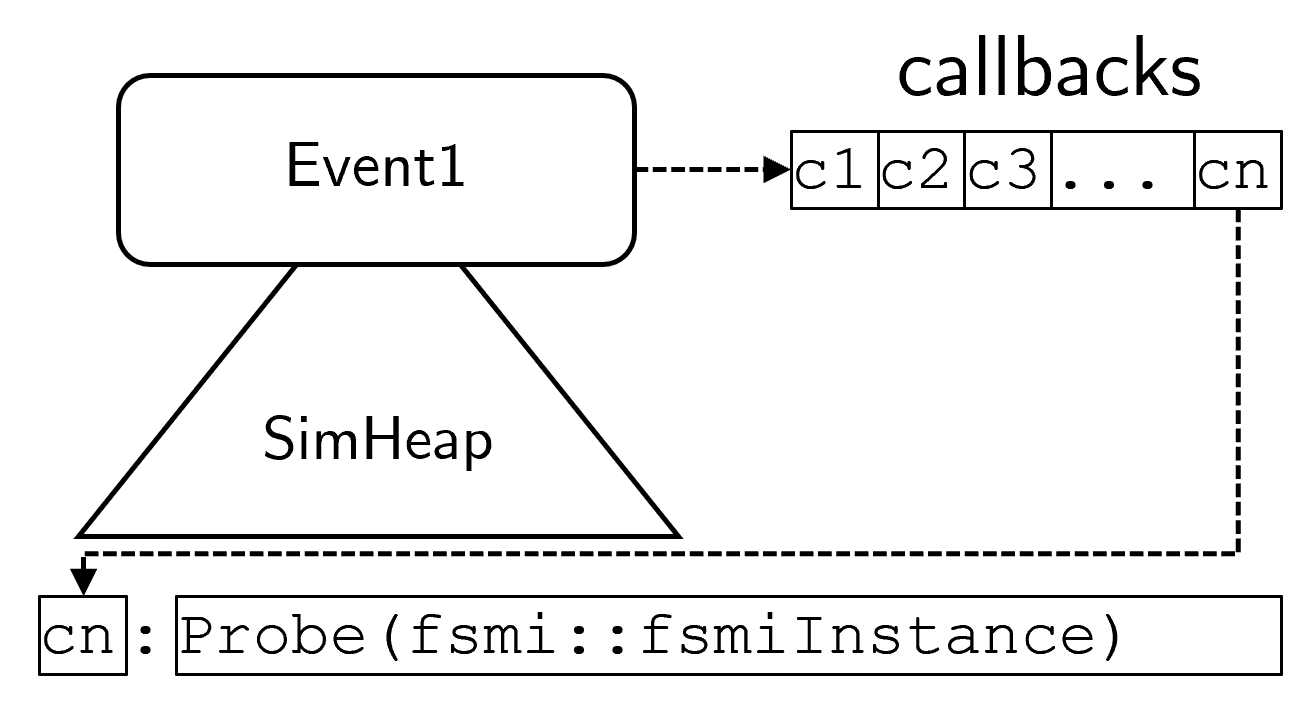
\includegraphics[width=0.9\linewidth]{images/simHeapCallbacksProbe}
	\caption{Event callback functions: probing}
	\label{fig:cbprobing}
\end{figure}
 However, since active processes switch back and forth, the probe might collect a different set of variables after the occurrence of each event. For this reason the probe needs to be aware of the kind of the active process. The latter implies the need to pass the FSMI itself as an argument to the probing function. In its turn, this results in the correct set of state variables. This set gives rise to an object which includes the necessary fields for every process, which must be persisted to the database. \vskip 6pt

This is closely related to the definition of an ORM, which is the technique of choice to persist data. Often, ORMs have a static configuration to determine which objects can exist and to which relations and attributes they map. PostgresORM \cite{tecnivelPostgresORM} uses the same approach, using modules to achieve this. In our implementation, macro expansion is used to generate these modules dynamically at compile time. The concerned macros take as an input the configuration for an ORM and produce the PostgresORM compatible modules. As such, a dynamic ORM is realised. The probing function selects a suitable object instantiator function and persists the object in the correct relation due to the mapping module. Multiple simulation runs can benefit from the same macro expansion.\vskip 6pt

To retrieve the necessary input which drives these macros, we must analyse the model under consideration. It is however unnecessary to execute the analysis prior to each simulation run. If the simulation model remains unchanged, the data model, hence the state variables that need to be persisted remain stable as well.\vskip 6pt

\texttt{ResumableFunctions.jl} performs such an analysis at compile time due to the \texttt{@resumable} macro. Our architecture benefits from this implementation to retrieve and store the simulation model's metadata. This model metadata is stable and needs to remain available throughout several simulation runs and must therefore be persisted separately. Therefore, a classic usage of a static ORM is suitable in this case.\vskip 6pt

The inner workings of our novel architecture described so far lead to an implementation in three phases, which require distinctive infrastructure to be foreseen:

\begin{enumerate}
	\item In a first phase, the simulation model is analysed. Static programming logic and infrastructure is used to retrieve and hold model metadata for internal exploitation.
	\item In a second phase, the dynamic ORM is realised through macro expansion, driven by the metadata gathered in the first phase. To persist data, dynamic infrastructure, dependent on the model under consideration is created and used to persist data.
	\item In a third phase data is made externally available using the data model which was created in the previous phase. A REST API and a \texttt{vue.js} data interface are provided.
\end{enumerate}

Figure \ref{fig:threePhase} shows these three phases, together with the main functions and modules that are used within it. In the following, we will explain how these three phases are implemented in terms of programming logic and database configuration.

\begin{figure}[th]
	\centering
	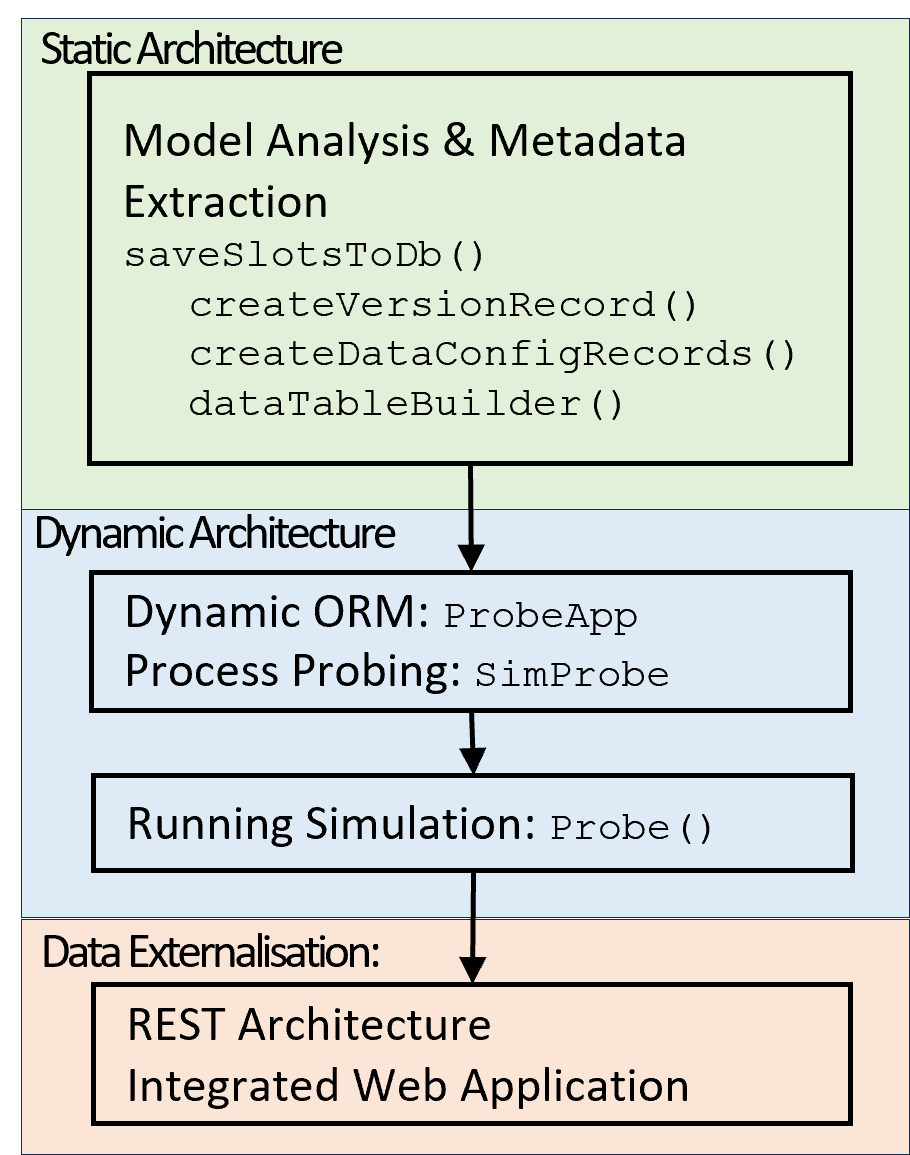
\includegraphics[width=0.6\linewidth]{images/threePhase}
	\caption{Three phased approach}
	\label{fig:threePhase}
\end{figure}

\subsection{Static Architecture}\label{statArch}

The starting point for each simulation is the definition of the model as resumable functions. We benefit from this macro expansion step to store the extracted information about the state variables (slots), present in the function. For this purpose, we extended \texttt{ResumableFunctions.jl} in two ways: (1) the macro now additionally saves metadata about the model itself and the slots present in each process and (2) takes a second boolean argument either to persist or not the evolution on the state variables. %The latter merely adds the process's friendly name to a globally defined array which is used to communicate to the probe. That way the function "announces" itself as a monitored function.

\vskip 6pt

The \texttt{@resumable} macro internally depends on the existing \texttt{get\_slots()} function. Here, we introduced our new \texttt{saveSlotsToDb()} function which (1) saves information about the version of the model through the function \texttt{createVersionRecord()}, (2) saves the configuration of these slots to the database through the \texttt{createDataConfigRecords()} function and (3) creates the relations that will hold the data for the function/process under consideration through the \texttt{dataTableBuilder()} function. \vskip 6pt

The function \texttt{createVersionRecord()} creates a \textit{modelmetadata} record in a dedicated relation, only if the model did not exist before. In the other case the concerned record gets updated. 
%For this purpose, such a record includes the friendly name of the initiating model-function (which was the argument to the \textit{@resumable} macro), the hash of that function, along with timestamps to keep track of the creation time and last used time in the simulation model. 
The primary key for such a process (and therefore also of the \textit{modelmetadata} record) is the function name (that was originally passed to the \texttt{@resumable} macro), along with a hash of the slots. The relation holding information about the process under consideration includes the attributes name, hash of the slots, UUID, model creation timestamp and last used timestamp. To store the data, a static ORM was defined which is used to query the relation for the primary key of the process under consideration. Should the key exist, then the last used timestamp gets updated. Otherwise, a record gets created. \vskip 6pt

After having saved the metadata concerning the current process, more fine-grained metadata concerning the process's specific slots is saved through the \texttt{createDataConfigRecords()} function. This function provides the necessary information to the macros that create the dynamic ORM. In the dedicated \textit{objectclassdefinition} relation, each slot's metadata is stored to feed these macros: object and relation name, the object's field name, the data type, the mapping attribute and information whether the field participates in a primary key or not. This is realised through two static ORM definitions which point to the same relation. \vskip 6pt

Both of the relations we considered so far are statically defined. The attributes are known upfront, which allowed for a static ORM and an unvarying SQL DDL statement. The relation necessary to persist the slots of a process during the simulation is different since the attributes may vary depending on the slots present in the process. Therefore a dynamic SQL DDL statement needs to be established and executed for each new process. This is the task of the \texttt{dataTableBuilder()} function which builds and executes the SQL DDL for each process. We benefit from the SQL \texttt{IF NOT EXISTS} constraint to skip the creation for tables that already existed due to prior simulations of a certain process, including a same set of slots. \vskip 6pt

The architecture requires a PostgreSQL database instance running with a dedicated schema present. The schema must contain both of the statically defined relations: \textit{modelmetadata} and \textit{objectclassdefinition}. Access must be granted to a specific user for connections from static and dynamic ORM definitions. The schema holds the dynamically defined relations as well. \vskip 6pt

\subsection{Dynamic Architecture}

Given the availability of model and processes metadata, the probing and persistence of a running simulation model is possible by using that metadata in the dynamic part of our architecture. The starting point is the newly added \texttt{@runPersisted} macro to \texttt{ConcurrentSim.jl}, which must be used to start a simulation  instead of the \texttt{run()} function, which remains available as well. The newly added macro performs two functions: (1) it includes the \texttt{ProbeApp} module which is a dynamically created module, dependent on the gathered metadata and (2) designates which dynamic ORM provided object instantiator functions are used to probe which processes. \vskip 6pt

\subsubsection{The ProbeApp Module}\hfill\\

\texttt{ProbeApp} is the module which implements the internal \texttt{Model} and \texttt{ORM} modules that make up a standard PostgresORM configuration. Both of them are implemented as macro calls: \texttt{@makeObjectDefModule} and \texttt{@makeOrmDefModule} respectively for Model and ORM creation, at the same location you would configure PostgresORM statically. These macros share the design principle that they both exploit metadata collected in the static part of the architecture described in section \ref{statArch} , which alters the standard static approach of PostgresORM to the novel dynamic behaviour.\vskip 6pt

%\paragraph{\textnormal{\texttt{@makeObjectDefModule}}}\hfill\\
\paragraph{The makeObjectDefModule Macro}\hfill\\

The aim of \texttt{@makeObjectDefModule} is to build a PostgresORM-compliant module containing object definitions synthesised from the records available in the objectclassdefinition table. The task is accomplished by building an expression which evaluates to the \texttt{Model} module which configures PostgresORM. The object definitions included in this expression are created through mapping the \texttt{objToObjDef} over an array of metadata objects which originated from the table. Only the attributes of interest are retained in the record to metadata-object translation. The same static ORM we used previously to store data in the concerned table is now used to query it. A secondary task of the macro is to identify the current model's instantiator functions, since the probe will use only these later on. These are added to an array which becomes available in the global scope after evaluation of the macro. \vskip 6pt

\texttt{objToObjDef} realises individual struct definitions. It does so for what is concerned the fields of the struct by means of string interpolation in a quoted expression. Further, the function also uses \mbox{\texttt{MacroTools.jl}'s} \texttt{combinedef()} to generate both of the necessary positional and keyword constructor functions to comply with \mbox{\texttt{PostgresORM.jl}'s} requirements. As such, \texttt{objToObjDef()} is an aggregating function on the metadata objects.

%\paragraph{\textnormal{\texttt{@makeOrmDefModule}}}\hfill\\
\paragraph{The makeOrmDefModule Macro}\hfill\\

The inner workings of \texttt{@makeOrmDefModule} are very similar to \texttt{@makeObjectDefModule}. The macro evaluates to an \texttt{ORM} module which is internal to PostgresORM and works in tandem with the object definition created through the evaluation of the \texttt{@makeObjectDefModule} discussed earlier. Each object definition requires the corresponding ORM.\vskip 6pt

Metadata objects resulting from the \textit{objectclassdefinition} table serve as an input to the function \texttt{createOrmsFromDB}, which generates the ORM modules dynamically on a per-object basis. The final module body is generated through string interpolation in a quoted expression.

\subsubsection{The SimProbe Module}\hfill\\

Probing and persistence is realised through the \texttt{SimProbe} module, which exports the probing function, and acts upon the different (sub)processes. As illustrated in Figure \ref{fig:cbprobing}, the probing function is activated through inclusion in the array of callback functions which get executed when an event occurs. \vskip 6pt

\paragraph{Probe Implementation}\hfill\\

The \texttt{SimProbe} module implements the \texttt{ProbeStructured()} probing function which takes the FSMI instance as an argument. To comply with \texttt{ConcurrentSim.jl}, a wrapper function \texttt{Probe()} exists as well. A mapping dictionary available at the main simulation environment struct provides the information whether the FSMI instance under consideration is truly a monitored process through the presence of the corresponding object instantiator function. The probing function transfers the variables present in the FSMI to a corresponding struct. The latter is then persisted to the database. This mechanism relies entirely on the availability of the dynamic ORM which is available in the global scope through macro expansion from within the module \texttt{ProbeApp}, and on the coupling of FSMI types to the correct instantiators.\vskip 6pt

\paragraph{Probe Activation}\hfill\\

The \texttt{Probe()} function is activated using the array of callback functions. The evolution of the variables in a running simulation maps to the evolution of the state variables in the corresponding state machine. The latter is a representation of a (sub)process contained in the simulation model. To capture state variables, the full array of callback functions must be executed first. Only then, a state machine can make a transition from one state to another, or in other words, proceed to the next event. We added the \texttt{probe} function as a callback function.\vskip 6pt

Finally, the probing aspect and the dynamic ORM aspect are joined together through the coupling of the type of FSMI to the correct instantiator. This is only possible when the static phase has terminated, and the dynamic phase is beyond the evaluation of the \texttt{SimProbe} module. At this moment, the information is available which functions must be monitored, and how their ORMs should look like. Furthermore, through the dynamic phase, the necessary ORMs are in place. At this stage, the ORMs are available to the \texttt{SimProbe} module to create and store shadow objects for each monitored process. The detailed overview is available in figure \ref{fig:detView}. This figure shows the static architecture which extracts and stores model metadata through an upfront known ORM definition and then dynamically generates the ORMs based on that metadata. Object definitions and persistence api are now available on a per-process basis.

\begin{figure}[th]
	\centering
	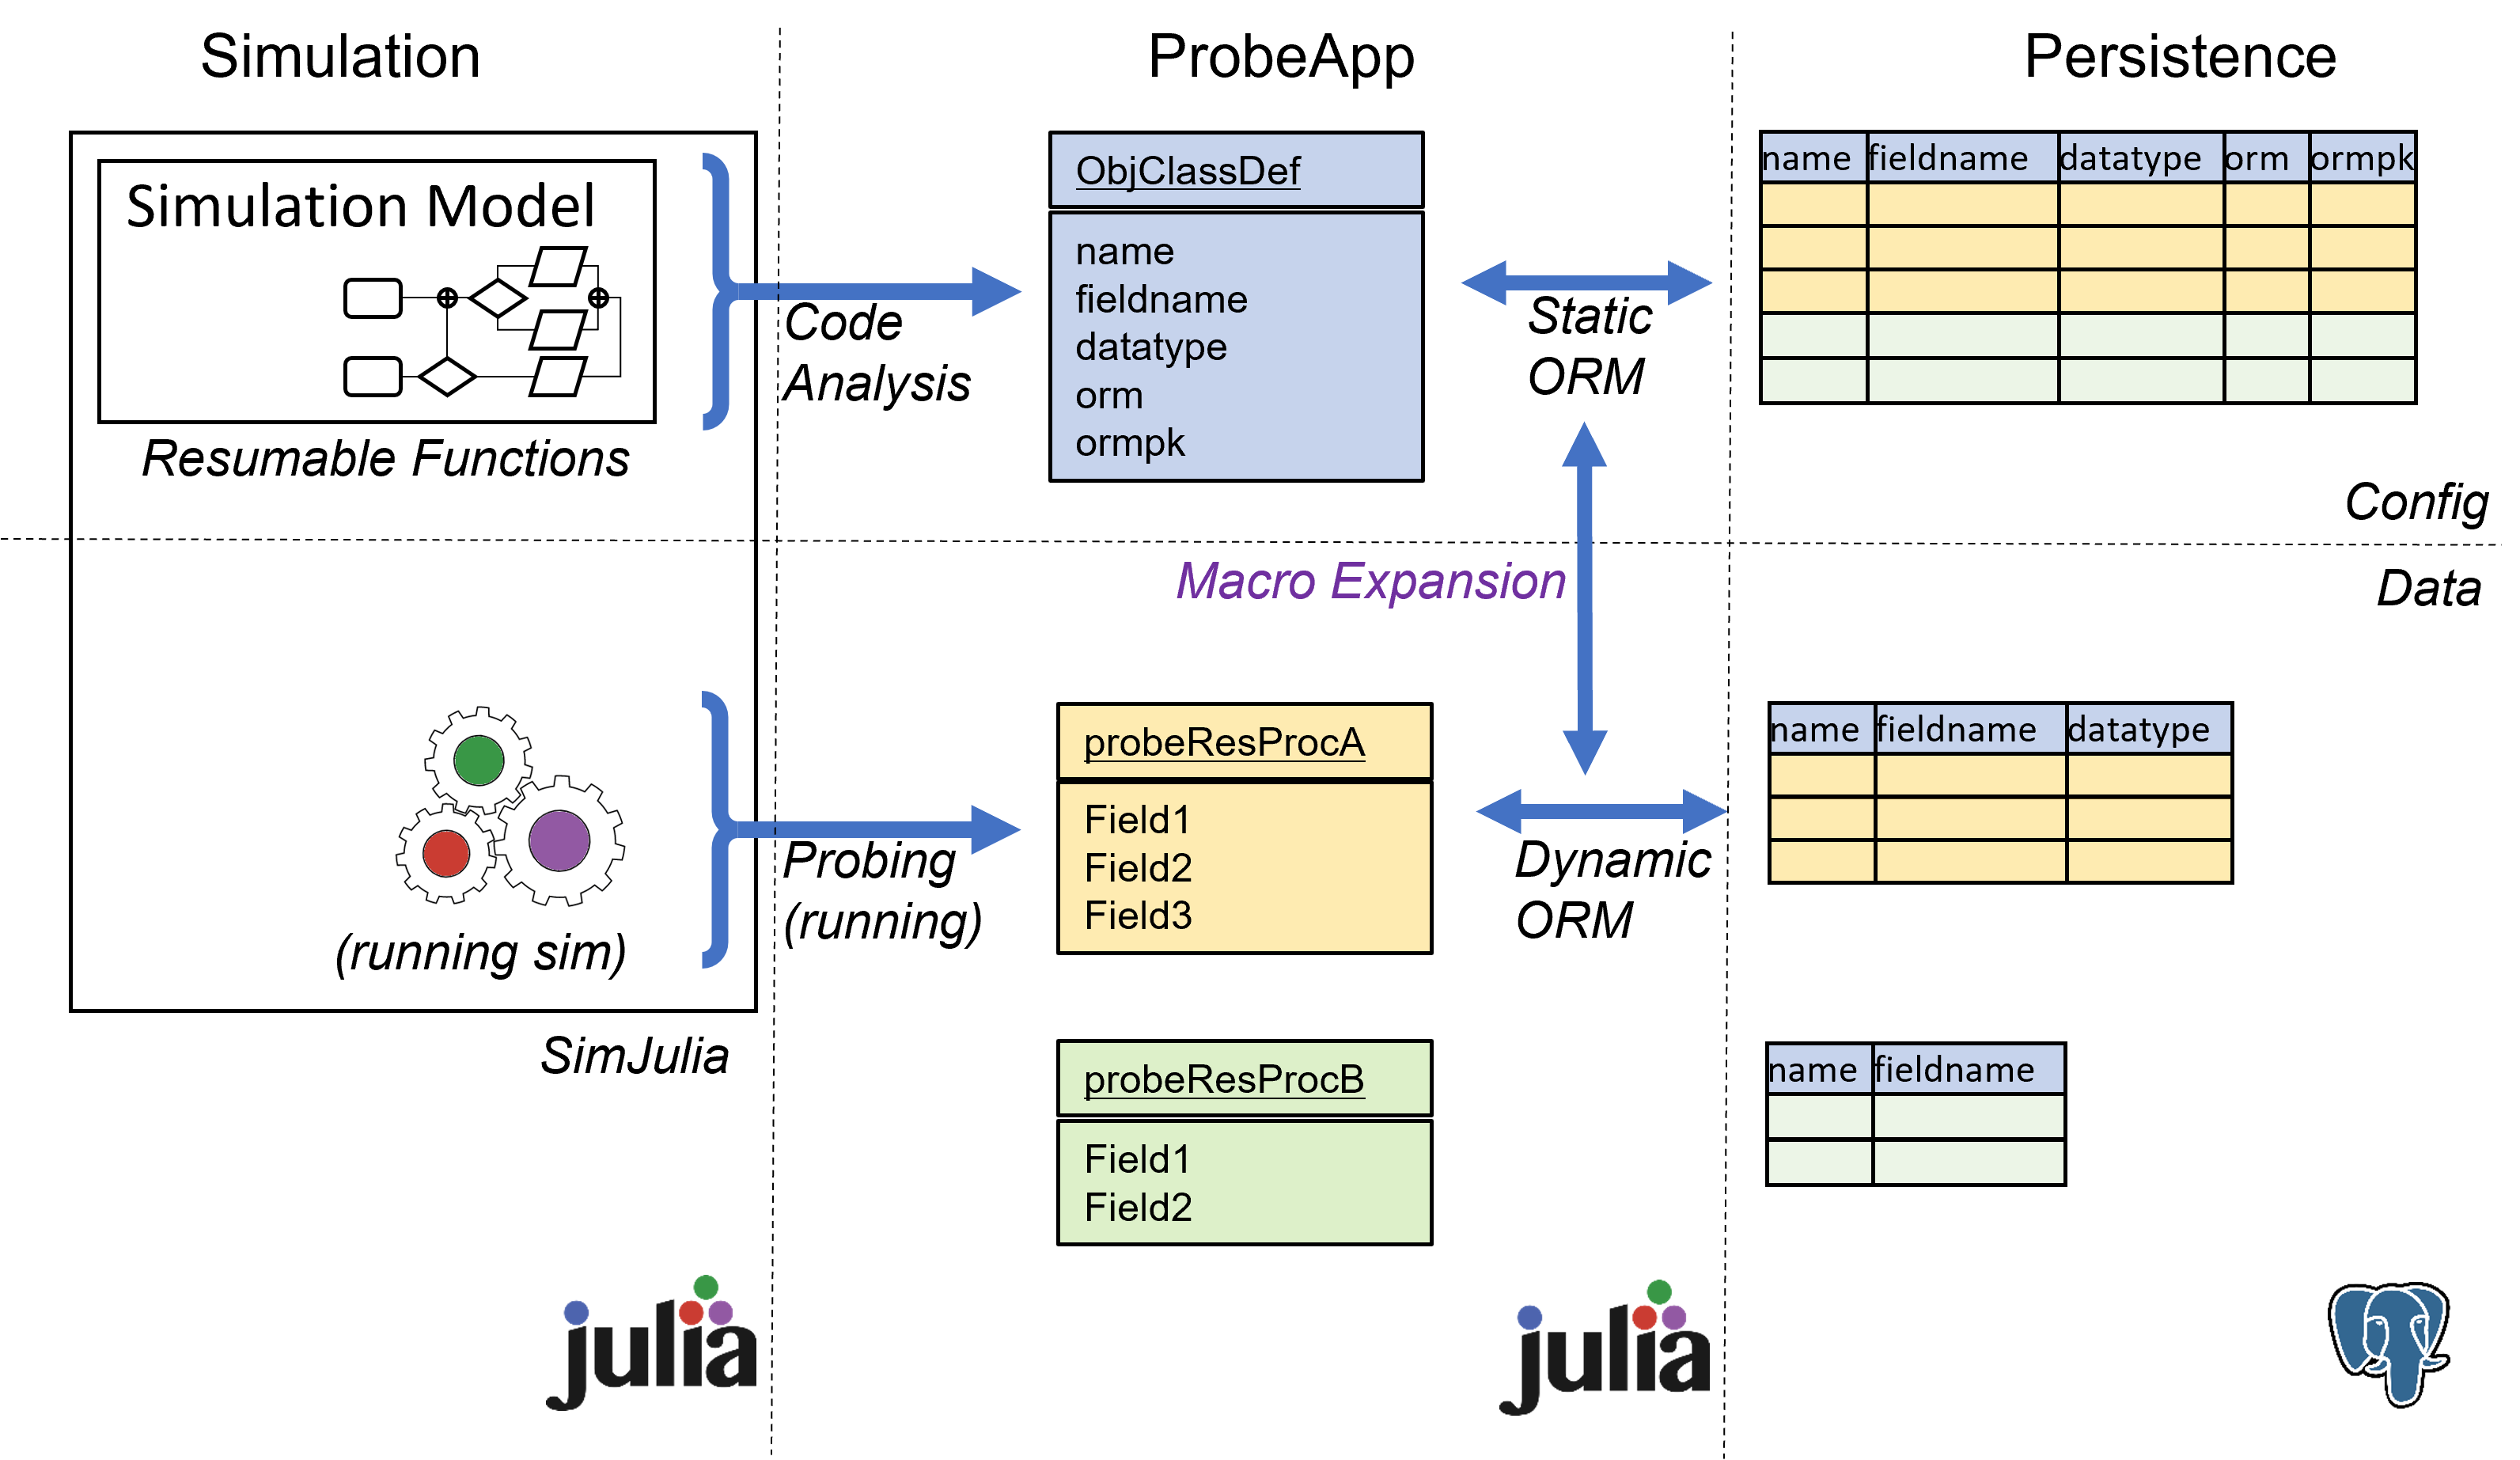
\includegraphics[width=1\linewidth]{images/overviewArch}
	\caption{Detailed Architecture}
	\label{fig:detView}
\end{figure}

The coupling of the type of the FSMI to the instantiator is executed just before the simulation starts. The newly added \texttt{@runPersisted} macro performs this function. It iterates over the globally defined array of processes that need to be monitored (those who ''announce'' themselves) and designates instantiator functions to FSMI types. This information is stored at the top-level simulation environment struct which was extended for this purpose.\vskip 6pt

\subsection{Data Externalisation}

To externalise the data gathered using the techniques described earlier, we devised two distinct approaches which share the same goal: a user should have access to all persisted data, either through an interface implementing an open standard, or in tabular format from within a web browser. The first approach consists of a REST architecture, while the second approach is an integrated solution which includes a web application running in a single thread, mainly based on the \texttt{VueJS.jl} package. \vskip 6pt


\subsubsection{REST Architecture}\hfill\\

The REST architecture consists of a Julia implementation of the REST API using the \texttt{HTTP.jl} package. A HTTP server listens at a given port for a request for a virtual directory. The required table, which maps to a monitored process, is then passed to the server as a virtual directory in the requested URL, and gets extracted using the positional pattern matching features provided by the \texttt{HTTP.jl} package. Together with the HTTP GET method, the server is aware the request is a READ operation on a certain table.\vskip 6pt

The base implementation is highly inspired by the Cross-Origin Resource Sharing (CORS) example from the \texttt{HTTP.jl} documentation \cite{httpjl}. However, in our implementation, a request arriving at the server invokes a \texttt{getTableContent()} service function which will request the data from the back-end database. Since the \texttt{ProbeApp} module is imported in the global scope where the HTTP server runs, and the required table was passed as a positional parameter (virtual directory) in the URL, we are able to instantiate the correct filter object for the required table and pass it to the ORM's \texttt{retrieve\_entity()} function. The resultset is then transformed to the correct JSON format using the \texttt{JSONMiddleware} and \texttt{CorsMiddleware} functions provided by the documentation. These two functions implement the CORS-oriented aspects as well. For the inner workings of the two latter functions, we refer to the documentation.\vskip 6pt

\subsubsection{Integrated Web Application}\hfill\\

A router is defined in a global scope, on which several routes are registered. Such a route consists of a combination of a requested virtual directory and one of the HTTP request modes. When requested, a route invokes a function which returns a well-formatted html page which gets served upon the request arriving from a http client.\vskip 6pt

The \texttt{VueJS.jl} package intervenes in the local scope of such a function, exposing several html elements enriched by the original \texttt{Vue.js} framework. Apart from some static definitions, our application is centred around two functions. \texttt{showDataTables()} implements the landing page and shows a list of processes which corresponds to all processes ever persisted in the connected schema. Figure \ref{fig:vApplanding} shows an example of the landing page for the simulation model used throughout this text. Upon selection of a process, a parametrised http GET request is made against the HTTP server invoking the \texttt{showTable()} function. The latter builds the page containing the appropriate data table.

\begin{figure}[th]
	\centering
	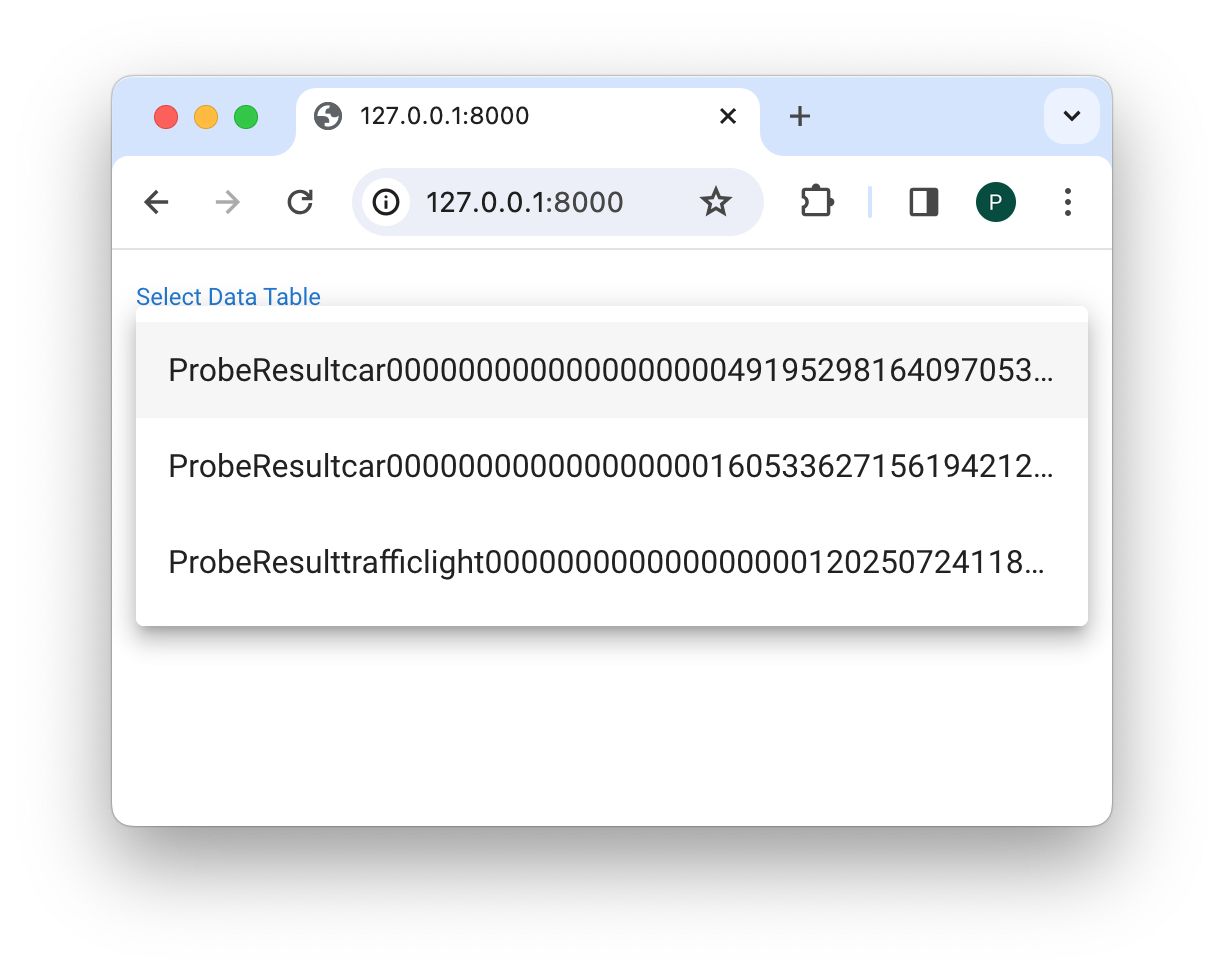
\includegraphics[width=0.9\linewidth]{images/VueApp}
	\caption{Integrated web application landing page}
	\label{fig:vApplanding}
\end{figure}

Our contribution is situated at the level of these two functions. They integrate our earlier, both statically and dynamically defined ORMs. Whereas these ORMs had a role towards data persistence earlier, they are  now employed in data retrieval. To do so, the \texttt{ProbeApp} module is imported in an application's global scope. \texttt{showDataTables()} uses the static ORM to retrieve the list of processes available in the schema. To do so, an unconfigured filter object is sent to the schema. The result is used to populate the list of possible processes at the landing page. As selection of one of these processes invokes the \texttt{showTable()} function which is aware of what kind of filter object to send to the schema.\vskip 6pt

Since \texttt{VueJS.jl} is highly oriented towards dataframes, as implemented by \texttt{DataFrames.jl}, and the ORM's return a resultset comprised of objects, a utility function bridges the gap between the two. It allows to send any filter object to a schema, and receive the appropriate dataframe in return.\vskip 6pt

\section{Technical Evaluation}

The architecture, which is available at \url{https://github.com/vanderpp/ResumableFunc}, was validated using several scenarios reflecting the intended use during simulations. We used a MacBook Pro, equipped with an Intel Core i5-5257U processor with 8GB RAM. We used VSCode v1.84 with Julia v1.8.5. \texttt{PostgresORM.jl} is at v0.5.0. The changes to \texttt{ResumableFunctions.jl} were implemented starting off from v0.6.3 and for \texttt{ConcurrentSim.jl}  we started working on v0.8.1. The RDBMS is PostgreSQL v13.13. The simulation which was used to run the test cases can be found at \url{https://github.com/vanderpp/ResumableFunc/blob/master/test_SimProbe.jl}\vskip 6pt

\subsection{Inital Run}

The first group of scenarios cover metadata generation and initial simulation runs. We ran the simulation model with both the \texttt{car} and \texttt{trafficlight} processes unmonitored, which resulted in alterations in the modelmetadata and objectclassdefinition tables. In the first table, records are added which indicate the same model "creationtime" and "lastused" timestamp. In the second table, the object metadata to feed the dynamic ORM creation macro's are present. No data was recorded, as expected. A subsequent run of the model altered the "lastused" timestamp as expected. We conclude these scenarios led to the expected outcome. \vskip 6pt

Having run the scenarios directed towards metadata generation, a subsequent series of scenarios directed towards data generation were run. The preconditions for these scenarios were either none, or having run the metadata scenarios. For this purpose, the \texttt{car} and \texttt{trafficlight} processes were set to "monitored", which, upon evaluation of the model, resulted in the creation and population of the corresponding data tables. All possible variations on which process was monitored during simulation were explored, with conclusive results. \vskip 6pt

\subsection{Successive Runs}

Starting off from a model which had run previously, we devised a scenario where successive runs of the same, non-altered model, were evaluated. In the metadata tables, the "lastused" timestamps were updated with every run. The corresponding data tables got appended newly generated data, distinguishable from earlier runs through the "simulation start time" attribute.\vskip 6pt

Next, an existing simulated model with persisted data was altered to evaluate the detection of the alteration, and to observe the creation of new metadata records. Furthermore we expect new data tables accommodating the altered model data. The result for this scenario was positive. Continuing this scenario, we reverted back to the pre-existing scenario which resulted in the priorly existing data tables to get appended with the new data, generated by the reverted model. \vskip 6pt

\subsection{Data Externalisation}

The starting conditions for this scenario is to have a simulation that has run, and data was recorded. The REST endpoint is queried using a HTTP GET request  at the URL: http://127.0.0.1:8001/api/tablecontent/<tableName> where <tableName> must be replaced with the real table name containing the data.\vskip 6pt

The integrated web application is reachable at the IP address the HTTP server was started on. At the landing page, a drop down list was filled dynamically from the available metadata. Such a landing page example is depicted in Figure \ref{fig:vApplanding}. This allows for the selection of any of the available process's data.\vskip 6pt

\subsection{Performance Comparison}

Using the \texttt{@time} macro, we recorded the elapsed time for simulations started with the new \texttt{@runPersisted} macro. To compare performance, a series of twenty measurements was taken in each of the following configurations: non-persisted configuration (nn), persisted configuration (np). Lastly, we also took measurements using the prior method to start simulations using the \texttt{run} function (on). All of these scenarios are based on our standard simulation. \vskip 6pt

This lead to the following mean elapsed times: $\overline{t}_{nn}=0,0342 s$,  $\overline{t}_{np} = 7,2781 s$ and $\overline{t}_{on} = 0,276 s$. We observed a difference in means using ANOVA ($\alpha = 0,05$, $p<0,001 $). Multiple comparisons (Fisher LSD with Bonferroni) revealed a homogeneous group amongst $t_{nn}$ and $t_{on}$. When used in the persisted configuration (np), our architecture is significantly ($p < 0,001$) slower when compared to the non-persisted configuration (nn).


\vskip 6pt

\section{Discussion}

The starting point for our architecture was the absence of a persistence architecture in \texttt{ConcurrentSim.jl} and the underlying \texttt{ResumableFunctions.jl} packages. Currently we rely on the knowledge of the user on persistence technology to implement this aspect. From our experience, we know the presence of that knowledge is a strong assumption. More importantly, in many cases the assumption is not true. Therefore, we wanted to integrate a fully automated solution for persistence in \texttt{ConcurrentSim.jl} and \texttt{ResumableFunctions.jl} with minimal user intervention. We identified two distinctive parts in the problem to which our architecture is the solution. Firstly, the data needs to be extracted from the running simulation. Secondly, this data must be persisted for later use. The solution should require a minimum of configuration and infrastructure, since our main goal is to relieve the user of any of such burdens.\vskip 6pt

For what concerns the data extraction, we must decide when the probing function should be executed. It seems obvious the right time is the instant prior to the transition from one state to the next state. In ConcurrentSim, this is after the execution of an event which is the trigger to execute the callback functions. Therefore, ConcurrentSim's \texttt{execute} function was altered to schedule a callback function, which is the Probing function. \vskip 6pt

The probing function is exported by a module \texttt{SimProbe} which is imported into ConcurrentSim. \texttt{SimProbe} on its turn imports the \texttt{ProbeApp} which is in fact the encompassing ORM module which includes the domain objects and the persistence API. Both are generated dynamically using macro expansion, driven by the metadata which was collected during the evaluation of the ResumableFunctions macros. \vskip 6pt

Due to the approach we took to extract metadata to drive the macros which generate the ORM modules, and the requirement to hide the model analysis phase from the running simulation phase, which is probed in the background, we introduced the risk for a world age problem. This risk is situated at the moment we want to load the module which provides the probing function with the object instantiators to persist data using the dynamic ORM. This can only be after the model analysis took place. So in the simulation application you would need to include the \texttt{using SimProbe} statement after the model declaration, and just before the \texttt{run} function call. This is cumbersome, so we decided to hide that as well using a \texttt{runPersisted} macro which essentially loads the probing module when model metadata is available and before the probing function is scheduled as a callback.\vskip 6pt

The newly introduced architecture comes at a performance cost. Statistical analysis of the elapsed times for both persisted and non-persisted scenarios revealed the introduction of a non-negligible delay in the simulation process. Persisting the simulation data causes I/O which takes additional time. Improvements can be made at that level by introducing some buffering mechanism. \texttt{PostgresORM.jl} provides the possibility to flush an array of objects to the database. That approach was not explored but seems promising. Another possibility would be to run the database in-memory to reduce the I/O overhead. \vskip 6pt

With regard to the decision when to consider a process as "altered" from the previous version during successive simulations, we took the approach in which the name of the function that describes the process together with the hash of the array containing the local variables of such a process determines the unicity of a process. As a consequence, when the semantic meaning of a process changes, this is not recorded in the persistence tier of our architecture. It can however be circumvented by annotating the process using a variable. This approach is exploited to associate the right object instantiator in the global context of the simulation application with a version of a process. When the probing function is invoked, it uses this information to decide which object to create and persist.\vskip 6pt

Prior to the decision to integrate \texttt{PostgresORM.jl} in our architecture, several approaches were explored. The most noteworthy were the option to use \texttt{SearchLight.jl} and a proper ORM. \texttt{SearchLight.jl}, which is the dedicated ORM back end for \mbox{\texttt{Genie.jl} \cite{genie}} has the advantage it is an evolved package, used and supported by a user community. Relevant in size, however, in our opinion it is tightly coupled to Genie. The way it is implemented (using separate modules for each object and the concept of migrations to create the tables), lead to a preference for \texttt{PostgresORM.jl}. The approach to create our own ORM was explored profoundly, and lead to the conclusion to cease that approach due to development time cost, and typical quality of code realised in such approaches. \texttt{PostgresORM.jl} gained the preference due to its straightforward approach of the domain objects module and the persistence API. We saw an ideal combination in the capabilities of macro expansion in Julia together with the \texttt{MacroTools.jl} package, driven by external metadata to generate the modules dynamically at compile time.\vskip 6pt

The REST API that we implemented opens up the possibility to process and analyse the generated data using an external (web)application. During the implementation, we encountered the need to implement the Cross-Origin Resource Sharing solution, since it is not guaranteed such an application runs at the same location the REST API runs. A simple REST implementation would suffice if only retrieving the JSON file would be the interest. However, our version support both the basic and richer approach. The \texttt{HTTP.jl} documentation proved itself very useful to implement this. A shortcoming of the REST API is that a user needs to know upfront the rendez-vous point. A page summarising the possible rendez-vous points could easily be implemented based upon the available metadata.\vskip 6pt

To provide the user with an immediately available web interface to explore the stored data, we devised an architecture involving VueJS, based on the ORM which was generated dynamically. In this scenario, there exists a landing page on which the user can select amongst the tables that exist in the database, hence the simulated processes that have been persisted. The user is taken to the concerned table where data is available for exploration. \vskip 6pt

A known limitation of our system is the absence of the possibility to exclude certain variables from the persistence. It is the consequence of the decision to streamline the integration of the analysis phase and the simulation phase. Should we desire to implement more fine-grained probing, the decision what to include in the "shadow-object" used for persistence must be taken between these phases. To be more precise, after the generation of the metadata which drives the dynamic ORM generation, but before the creation of the corresponding relations.\vskip 6pt

\section{Conclusion and Future Work}

Starting off from the observed shortcoming of ConcurrentSim to easily persist simulation data, and the requirement to provide such features without imposing additional knowledge requirements to the end user, we devised an architecture capable of persisting simulation data. The infrastructure and configuration requirements for using the presented architecture are minimal. The ConcurrentSim and ResumableFunctions packages were extended with modules that implement probing of a running simulation and persist it through a mechanism using a dynamically generated ORM. A running PostgreSQL instance is necessary, but the required configuration of that database schema is minimal as well. As such we were able to implement an architecture which fulfils the need. Furthermore, we implemented two data interfaces. The REST API allows for processing and exploration by external applications, while the VueJS application enables immediate data exploration from within a web interface. \vskip 6pt

The remaining challenges for end users could be further reduced or even completely avoided by incorporating our architecture in a web application which could accommodate the packages and architecture in an enclosed environment. Such an environment could facilitate model expression through a web interface. The same web application could provide an easy access to the data after the simulations have run. In that way, the remaining technical details could be hidden for an end user, whom at that point, could focus solely on the simulation task itself. \vskip 6pt

\bibliographystyle{juliacon}
\bibliography{ref}

%\vadjust{\vfill\pagebreak}
%% **************GENERATED FILE, DO NOT EDIT**************

\bibliographystyle{juliacon}
\bibliography{ref.bib}


\end{document}